\documentclass[conference]{IEEEtran}
\IEEEoverridecommandlockouts
% The preceding line is only needed to identify funding in the first footnote.
% If that is unneeded, please comment it out.
%\usepackage[backend=bibtex,style=verbose-trad2]{biblatex}

\usepackage{adjustbox}
\usepackage{algorithmic}
\usepackage{amsmath,amssymb,amsfonts}
%\usepackage[backend=bibtex,style=ieee]{biblatex}
%\usepackage{bookmark}
\usepackage{tabularx,array}
\usepackage{booktabs}
\usepackage{caption}
\usepackage{cite}
\usepackage{color}
\usepackage[inline]{enumitem}
\usepackage{float}
\usepackage[T1]{fontenc}
%\usepackage{fontspec}
\usepackage{footnote}
\usepackage{graphicx}
\usepackage[colorlinks=true,citecolor=blue]{hyperref}
\usepackage{inputenc}[utf8]
\usepackage{listings}
\usepackage{textcomp}
\usepackage[flushleft]{threeparttable}
\usepackage{subcaption}
\usepackage{xcolor}
\usepackage{cleveref}

\title{eBPF Computational Storage Device for ZNS in QEMU%\\
%{\footnotesize \textsuperscript{*}Note: Sub-titles are not captured in Xplore
% and should not be used}
%\thanks{Identify applicable funding agency here. If none, delete this.}
}

\pagenumbering{arabic}
\pagestyle{plain}

% Ensure decimal numbering in table  of contents
\renewcommand{\thesection}{\arabic{section}}
\renewcommand{\thesubsection}{\arabic{section}.\arabic{subsection}}
\renewcommand{\thesubsubsection}{\arabic{section}.\arabic{subsection}.\arabic{subsubsection}}

% ensure decimal numbering for sub sections
\makeatletter
\renewcommand{\@seccntformat}[1]{\csname the#1\endcsname.\quad}
\makeatother

% ------------------------------------------------------------------------%
% Proper Python Syntax Highlighting                                       %
% Author: redmode
% https://tex.stackexchange.com/questions/83882/how-to-highlight-python   %
% -syntax-in-latex-listings-lstinputlistings-command#83883                %
% ----------------------------------------------------------------------- %

% Default fixed font does not support bold face
\DeclareFixedFont{\ttb}{T1}{txtt}{bx}{n}{8} % for bold
\DeclareFixedFont{\ttm}{T1}{txtt}{m}{n}{8}  % for normal

% Custom colors
\definecolor{deepblue}{rgb}{0,0,0.5}
\definecolor{deepred}{rgb}{0.6,0,0}
\definecolor{deepgreen}{rgb}{0,0.5,0}

% Python style for highlighting
\newcommand\pythonstyle{
	\lstset{
		language=Python,
		basicstyle=\ttm,
		showstringspaces=false,
		tabsize=4,
		aboveskip=0.2cm,
		belowskip=0.2cm,
		otherkeywords={self},             % Add keywords here
		keywordstyle=\ttb\color{deepblue},
		emph={MyClass,__init__},          % Custom highlighting
		emphstyle=\ttb\color{deepred},    % Custom highlighting style
		stringstyle=\color{deepgreen},
		frame=tb,                          % Any extra options here
		prebreak=\textbackslash,
		linewidth=8.85cm,
		breaklines=true,
	}
}

% Python environment
\lstnewenvironment{python}[1][] {
	\pythonstyle\lstset{#1}
}{}

% Python for inline
\newcommand\pythoninline[1]{{\pythonstyle\lstinline!#1!}}

% Python for external file
\newcommand\pythonexternal[2][]{{\pythonstyle\lstinputlisting[#1]{#2}}}

% ----------------------------------------------------------------------- %

% Bash style for highlighting
\newcommand\bashstyle{
	\lstset{
		language=Bash,
		basicstyle=\ttm,
		showstringspaces=false,
		tabsize=2,
		%commentstyle=itshape,
		aboveskip=0.2cm,
		belowskip=0.2cm,
		prebreak=\textbackslash,
		extendedchars=true,
		mathescape=false,
		% literate= {\$}{{\textcolor{blue}{\$}}}1 {&}{{\textcolor{blue}{\&}}}1 {/n}{{\textcolor{green}{\textbackslash n}}}1,
		linewidth=8.85cm,
		breaklines=true
	}
}

% Bash environment
\lstnewenvironment{bash}[1][] {
	\bashstyle\lstset{#1}
}{}

% Bash for inline
\newcommand\bashinline[1]{{\bashstyle\lstinline!#1!}}

% Bash for external file
\newcommand\bashexternal[2][]{{\bashstyle\lstinputlisting[#1]{#2}}}


% Python style for highlighting
\newcommand\cstyle{
	\lstset{
		language=c,
		basicstyle=\ttm,
		showstringspaces=false,
		tabsize=4,
		aboveskip=0.2cm,
		belowskip=0.2cm,
		otherkeywords={self},             % Add keywords here
		keywordstyle=\ttb\color{deepblue},
		emph={MyClass,__init__},          % Custom highlighting
		emphstyle=\ttb\color{deepred},    % Custom highlighting style
		stringstyle=\color{deepgreen},
		frame=tb,                          % Any extra options here
		prebreak=\textbackslash,
		linewidth=8.85cm,
		breaklines=true,
	}
}

% Python environment
\lstnewenvironment{clist}[1][] {
	\cstyle\lstset{#1}
}{}

% Python for inline
\newcommand\cinline[1]{{\cstyle\lstinline!#1!}}

% Python for external file
\newcommand\cexternal[2][]{{\cstyle\lstinputlisting[#1]{#2}}}

% ----------------------------------------------------------------------- %

\begin{document}

\begin{titlepage}
\begingroup
\centering
{\LARGE\bfseries eBPF Computational Storage Device for ZNS in QEMU}

\vspace{1cm}

{\Large Vrije Universiteit (VU)}

\vspace{0.5cm}

{Corne Kenneth Lukken}

{\textit{Department of Computer Science} \\
Amsterdam, Netherlands \\
info@dantalion.nl}

\vspace{0.5cm}

\today

\vspace{4.0cm}

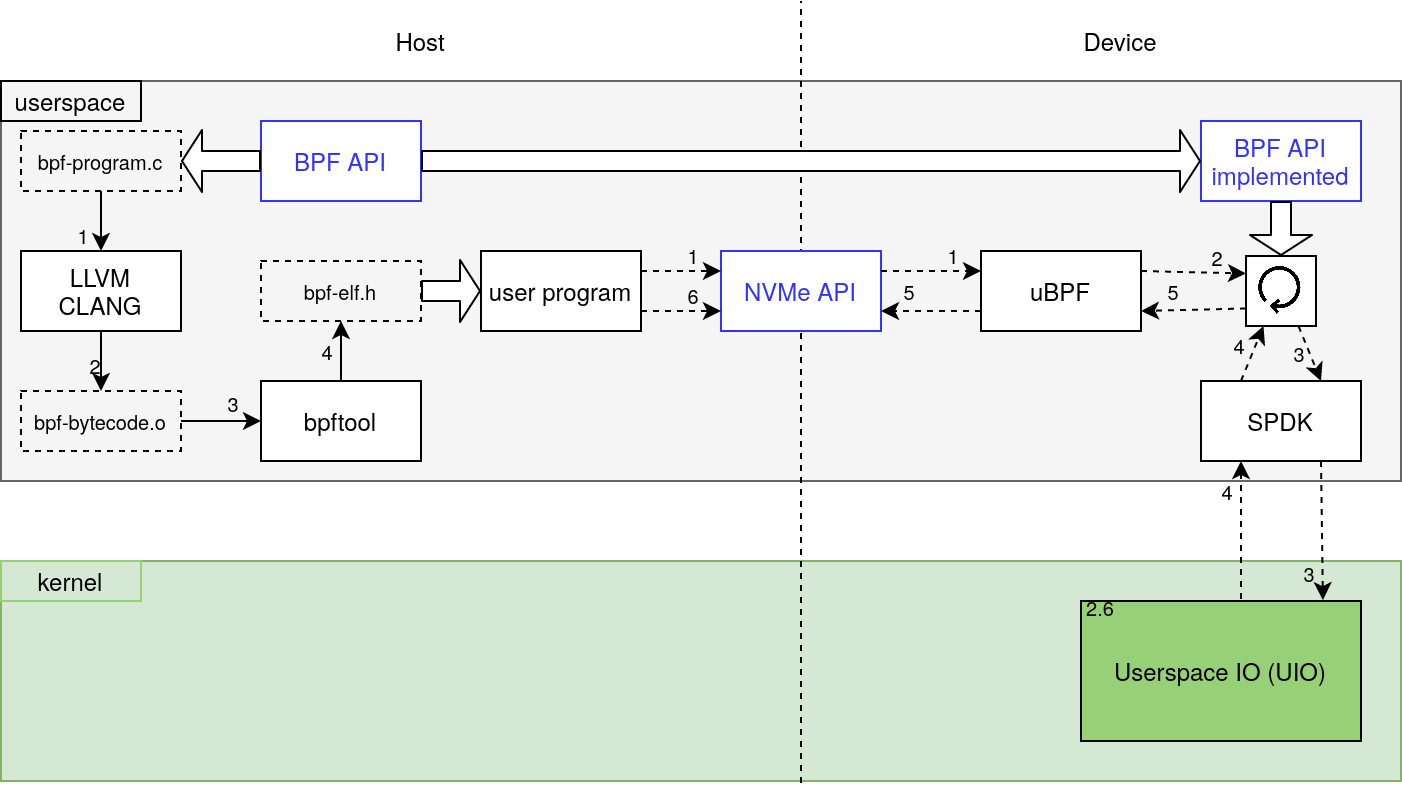
\includegraphics[width=0.8\textwidth]{resources/images/prototype-landscape.png}

\vfill
\endgroup
\begin{minipage}{0.4\textwidth}
	\begin{tabular}{ll}
		\Large Project course: & \Large Individual Systems Practical (X\_405088) \\
		\Large Supervisor: & \Large Giulia Frascaria and Animesh Trivedi \\
	\end{tabular}
\end{minipage} \hfill
\begin{minipage}{0.3\textwidth}
	\begin{flushright}
	
\includegraphics[width=\textwidth]{resources/images/vu-logo.png}
\end{flushright}
\end{minipage}
\end{titlepage}

\clearpage
\onecolumn

% Ensure black link color in table of contents
\hypersetup{
	linkcolor=black
}

\renewcommand{\contentsname}{CONTENTS}
\tableofcontents{}

\hypersetup{
	linkcolor=blue
}

\twocolumn

\addcontentsline{toc}{section}{\protect\numberline{}INTRODUCTION}
\section*{INTRODUCTION}

Recently pieces of literature have been presented about Zones Namespace (ZNS)
SSDs. These cover a variety of topics such as migrating from Open-Channel
SSDs (OCSSD) to Zoned Namespaces\cite{bjorling2019open}. Other literature
addresses some of the functionality these ZNS SSDs
introduce\cite{bjorling2020zone}. Finally, some works evaluate host-based SSD
features such as flash management and garbage collection when implemented using
ZNS SSDs\cite{254268,9188086}.

The concept of ZNS SSDs is interesting as this device level abstraction opens
new possibilities for research, such as for Computational Storage Devices (CSD).
Similar to OCSSD, ZNS gives insight into the internal device structure as well
as providing some additional guarantees. In the context of ZNS these structures
are known as namespaces and zones. This could have several advantages for CSD
applications as it could reduce the semantic gap between host and device.
Furthermore, it could provide safety guarantees by tying access level control
(ACL) to individual zones.

In order to investigate these research possibilities a functional prototype is
needed. The development of such a prototype requires making several decisions
such as to use existing technologies or develop new technologies. Typically,
from these technologies there might be several applicable options. furthermore,
the prototype might be aimed at answering a very specific research questions or
might be kept very broadly applicable intentionally.

In this work the use of ZNS SSDs as CSD will be investigated by building a
broadly applicable prototype. However, this requires the availability of ZNS SSD
devices. Currently, the availability of physical ZNS SSDs is problematic, this
is likely due to the NVMe Zoned Namespace technical proposal only being ratified
recently\cite{zns-nvme-ratified}. NVMe is the communication protocol prominent
across all flash based storage devices predominantly those connected using a
PCI-e bus.

This NVMe Zoned Namespace command set specification is what enables ZNS SSDs to
exist\cite{nvme-zns}. Luckily, the functionality of this NVMe command set is
already enabled in QEMU. QEMU is a dynamic binary translation emulator that
allows to create virtual hardware devices and subsequently use those inside the
emulator. This allows for the development of technologies utilizing ZNS SSDs in
a virtualized environment even if these devices do not currently physically
exist.

Several online resources exist explaining how this functionality was enabled in
QEMU\cite{nvme-qemu-1,nvme-qemu-2} as well as resources on general information
about ZNS SSDs\cite{zns-info}.

This work focuses on documenting the steps necessary to implement CSDs
utilizing ZNS SSDs with QEMU. The emphasis is on describing existing
technologies and how to combine these in a working prototype.

The overall structure of this work is as follows. Introduce several project
dependencies and how to configure these (\cref{dependencies}), describe
development and debugging methodologies and how these can be configured by
the CMake project accompanying this work (\cref{development}), describe the
existing technologies that are used in the final prototype (\cref{technology}),
define design requirements and the final implemented design as well as
limitations (\cref{design}), mention alternative technologies and why they
are not used in the prototype (\cref{alternatives}), finally, describe future
work and open questions that arise from this design (\cref{future}).

The entire prototype including source files for reports and documentation
is available online under an permissive open-source license\cite{qemu-csd}.

% \footnotemark[1]

% \footnotetext[1]{Time of writing is $10^{th}$ of February 2021.}

% \begin{center}
% 	\begin{figure}[H]
% 		\bashexternal{resources/bash/gitmodules.sh}
% 		\captionsetup{justification=centering}
% 		\caption{Contents of \textit{.gitmodules} file for this project.}
% 		\label{fig:example-gitmodules}
% 	\end{figure}
% \end{center}

\begin{table}[h!]
	\caption{BPF resources and their relevance}
	\label{table:bpfresources}
	\centering
	\begin{adjustbox}{width=0.5\textwidth}
		\begin{threeparttable}[]
			\begin{tabular}{lllll}
				\toprule
				\textbf{Resource} & \textbf{Category} & \textbf{Value} &
				\textbf{Length} & \textbf{Age} \\
				\midrule
				\href{https://www.man7.org/linux/man-pages/man2/bpf.2.html}{Linux bpf manpage}\cite{bpfman} &
				Linux Kernel & medium & short & timeless \\
				\href{https://www.kernel.org/doc/Documentation/networking/filter.txt}{BPF kernel documentation}\cite{Linuxbpf} &
				Linux Kernel & low & long & outdated \\
				\href{https://www.kernel.org/doc/html/latest/bpf/btf.html}{Linux BTF documentation}\cite{Linuxbtf} &
				Linux Kernel \& BTF & low & medium & timeless \\
				\href{https://facebookmicrosites.github.io/bpf/blog/2020/02/19/bpf-portability-and-co-re.html}{BPF portability and CO-RE}\cite{bpfport} &
				BPF CO-RE \& BTF & high & medium & relevant \\
				\href{https://nakryiko.com/posts/libbpf-bootstrap/}{BPF applications with libbpf-bootstrap}\cite{bpfapplications} &
				libbpf - libbpf-bootstrap & high & short & relevant \\
				\href{https://www.oreilly.com/library/view/linux-observability-with/9781492050193/}{Linux Observability with BPF}\cite{observabilityoreilly} &
				libbpf - bpf\_load & medium & book & outdated \\
				\href{https://facebookmicrosites.github.io/bpf/blog/2020/02/19/bpf-portability-and-co-re.html}{Cilium BPF + XDP reference guide}\cite{ciliumbpf} &
				libbpf & high & long & relevant \\
				\href{https://facebookmicrosites.github.io/bpf/blog/2020/02/20/bcc-to-libbpf-howto-guide.html}{BCC to libbpf conversion}\cite{libbpfconversion} &
				libbpf & low & long & relevant \\
				\href{https://github.com/iovisor/ubpf}{uBPF}\cite{ubpf} &
				execution / interpretation & medium & short & relevant \\
				\href{https://github.com/generic-ebpf/generic-ebpf}{generic-ebpf}\cite{generic-ebpf} &
				execution / interpretation & medium & short & relevant \\
				\bottomrule
			\end{tabular}
			\begin{tablenotes}[para,flushleft]
				\centering List of resources on BPF and its various elements.
			\end{tablenotes}
		\end{threeparttable}
	\end{adjustbox}
\end{table}

\section{Future Work} \label{future}

%\footnotemark[1]. example\ref{term}.
%\footnotetext[1]{test}
%\subsection*{Accelerated Computing Landscape}
%\textit{C++}
%GPUOCelot\cite{tired-manycore-architectures-ocelot}
%\section{LARGER SECTION}
%$\mathcal{O}(N\log N)$
%
%\begin{center}
%	\begin{figure}[H]
%		\bashexternal{resources/bash/inxi.sh}
%		\captionsetup{justification=centering}
%		\caption{Output of inxi showing both CPU and GPU hardware configuration}
%		\label{fig:inxihardware}
%	\end{figure}
%\end{center}

%\cite{Rius1995,Karp1996,parreverse,Adikaram2014}.

%\begin{center}
%	\begin{figure}[H]
%		\cexternal{resources/c/basic.c}
%		\captionsetup{justification=centering}
%		\caption{First basic kernel}
%		\label{fig:base}
%	\end{figure}
%\end{center}

\addcontentsline{toc}{section}{\protect\numberline{}TERMINOLOGY}
\section*{TERMINOLOGY} \label{term}

This section hopes to define some common terminology as well as clearly detail
how some of these terms are interpreted. Mainly, this section serves to avoid
confusion.

%\begin{tabularx}{\textwidth}{@{}l<{ -}@{\ }X@{}}
%	ZNS & Zoned Namespace \\
%	CSD & Computational Storage Device \\
%	Upstream & When a certain patch or feature has been \\ merged into the main
%		repository of a project. \\
%
%\end{tabularx}

\begin{enumerate}
	\item ZNS - Zoned Namespace
	\item CSD - Computational Storage Device
	\item ACL - Access Level Control
	\item Upstream - When a certain patch or feature has been merged into the
					 main repository of a project.
	\item GUI - Graphical User Interface
	\item IDE - Integrated Development Environment
	\item Target - A target is something that can be compiled or generated and
					 sometimes executed. Examples include PDFs using LaTeX,
					 binaries or libraries.
	\item Binary   - A binary is a file containing machine instructions that can
					 be directly executed. A compiled C file containing a main
					 method is a binary while a shell script is not. Typically
					 these binaries contain metadata information to aid the
					 underlying operating system in executing them, a common
					 format for this metadata is ELF.
	\item ABI      - Application Binary Interface.
	\item API      - Application Programming Interface.
	\item SCSI     - Small Computer System Interface
	\item ATA      - AT Attachment
	\item ZBC      - (SCSI) Zoned Block Command
	\item ZAC      - (ATA) Zoned ATA Commands
\end{enumerate}

\addcontentsline{toc}{section}{\protect\numberline{}REFERENCES}
\bibliographystyle{IEEEtran}
\phantomsection
\bibliography{bibliography}

\end{document}